\apendice{Documentación de usuario}

\section{Introducción}

\section{Requisitos de usuarios}

\section{Instalación}
A continuación se mostrarán los pasos a dar para instalar el software necesario.

\subsection{Osmosis}
La instalación de la herramienta Osmosis es sencilla. Una vez descargada la última versión, se ha de descomprimir en una carpeta a la que se tenga acceso de forma sencilla (por ejemplo: C:\textbackslash{}osmosis.
El aspecto del contenido de la carpeta será el reflejado en la Figura.

Para comprobar que Osmosis funcione de forma correcta se ha de abrir la consola de comandos y ejecutar el fichero de extensión bat que se encuentra en el interior de la carpeta bin.

Para abrir la consola de comandos de Windows desde la carpeta, simplemente se ha de pulsar la tecla shift y clicar el botón derecho del ratón en un espacio en blanco de la misma.

En caso de obtener algún error, consulta la página de referencia de Osmosis.

\subsection{PostgreSQL 9.6}

\subsection{PostGIS 2.0}

\subsection{RouteConverter}
Para poder usar RouteConverter en el ordenador se deberá acceder a la sección de descargas de su plataforma web: \url{http://www.routeconverter.de/downloads/es} y optar por la versión "Webstart". Esta versión está basada en Java resultando necesario contar con Java JRE instalado.

En la Figura se muestra la sección de descargas de la página. Para obtener la versión del programa deseada se ha de clicar sobre Webstart. Esto nos llevará a una nueva ventana mostrada en la Figura. Se ha de clicar sobre el botón naranja cuyo texto es "Launch". Por motivos de seguridad nos aparecerá un diálogo como el mostrado esta Figura. Aceptando el permiso de Java se descargará y lanzará la aplicación. La ventana principal luce como lo mostrado en la Figura.


\section{Manual del usuario}

\subsection{Osmosis}
Osmosis permite extraer una ciudad concreta de un mapa con formato pbf. En el caso de este trabajo, se ha descargado el mapa de España y se ha extraído la ciudad de Burgos. A continuación, se muestran los pasos a dar para obtener un fichero osm.

\subsubsection{Descarga del mapa de España}
Accediendo a la web de descargas de Geofabrik será posible elegir el país cuyo mapa que se desea descargar. Clicando sobre el enlace mostrado en la Figura, se puede descargar el mapa de España en formato pbf.

\subsubsection{Extracción de una ciudad}
Para extraer una ciudad del plano que se acaba de descargar, se ha de abrir la consola del sistema y hacer uso del fichero "getMap.bat". Se necesitarán los siguientes argumentos (entre paréntesis las coordenadas que serán usadas en el caso de Burgos):
\begin{itemize}
	\item Nombre de la ciudad: con esta cadena nombraremos el fichero osm de salida.
	\item Coordenada GPS que indique la parte superior del segmento de mapa que se va a recortar (42.658202).
	\item Coordenada GPS que indique la parte derecha del segmento de mapa que se va a recortar (-3.12561).
	\item Coordenada GPS que indique la parte inferior del segmento de mapa que se va a recortar (41.364442).
	\item Coordenada GPS que indique la parte izquierda del segmento de mapa que se va a recortar (-4.3066641).
\end{itemize}

El comando a teclear constará de lo siguiente:
\begin{itemize}
	\item rb: permite leer el contenido del fichero pbf descargado.
	\item bb: permite extraer los datos indicados en la caja definida por las coordenadas geográficas indicadas a continuación.
	\item top: coordenada geográfica superior.
	\item right: coordenada geográfica derecha.
	\item bottom: coordenada geográfica inferior.
	\item left: coordenada geográfica izquierda.
	\item wx: permite escribir los datos en un fichero osm.
\end{itemize}

Para la ciudad de burgos, el comando será el mostrado en la Figura. Ejecutando el comando se obtendrá el fichero "Burgos.osm".


\subsection{Uso de RouteConverter}

Una vez que se cuenta con este software en el ordenador, se pueden generar rutas o cargar ficheros con rutas ya definidas. En este caso se mostrará cómo cargar los datos de una ruta almacenada en la Base de Datos de Open Street Maps.

El primer paso a dar es la descarga de la traza que se desee visualizar con este programa.

\subsubsection{Descarga de ficheros gpx}
La descarga se realizará desde la página web de Open Street Maps, concretamente en la sección "Trazas". En esta sección se verán las últimas trazas subidas por los usuarios. Eligiendo una traza aleatoria accedemos a la ventana mostrada en la  Figura. Clicando sobre "descargar" se descargará el fichero gpx.

Estos ficheros contendrán una estructura XML con una serie de puntos geográficos que conformarán la ruta seguida por el usuario. La ruta podrá ser identificada con su nombre, el nombre del autor y una breve descripción.

\subsubsection{Carga de ficheros en RouteConverter}

Para cargar la traza en el programa, primero se debe abrir el software y después clicar sobre Archivo, Abrir. En la ventana emergente se ha de seleccionar la traza y clicar sobre Aceptar. En este momento se mostrará la ruta que describe la traza descargada desde Open Street Maps como se aprecia en la Figura \ref{rutaLeonFormigal}.

\begin{figure}[h]
  \centering
    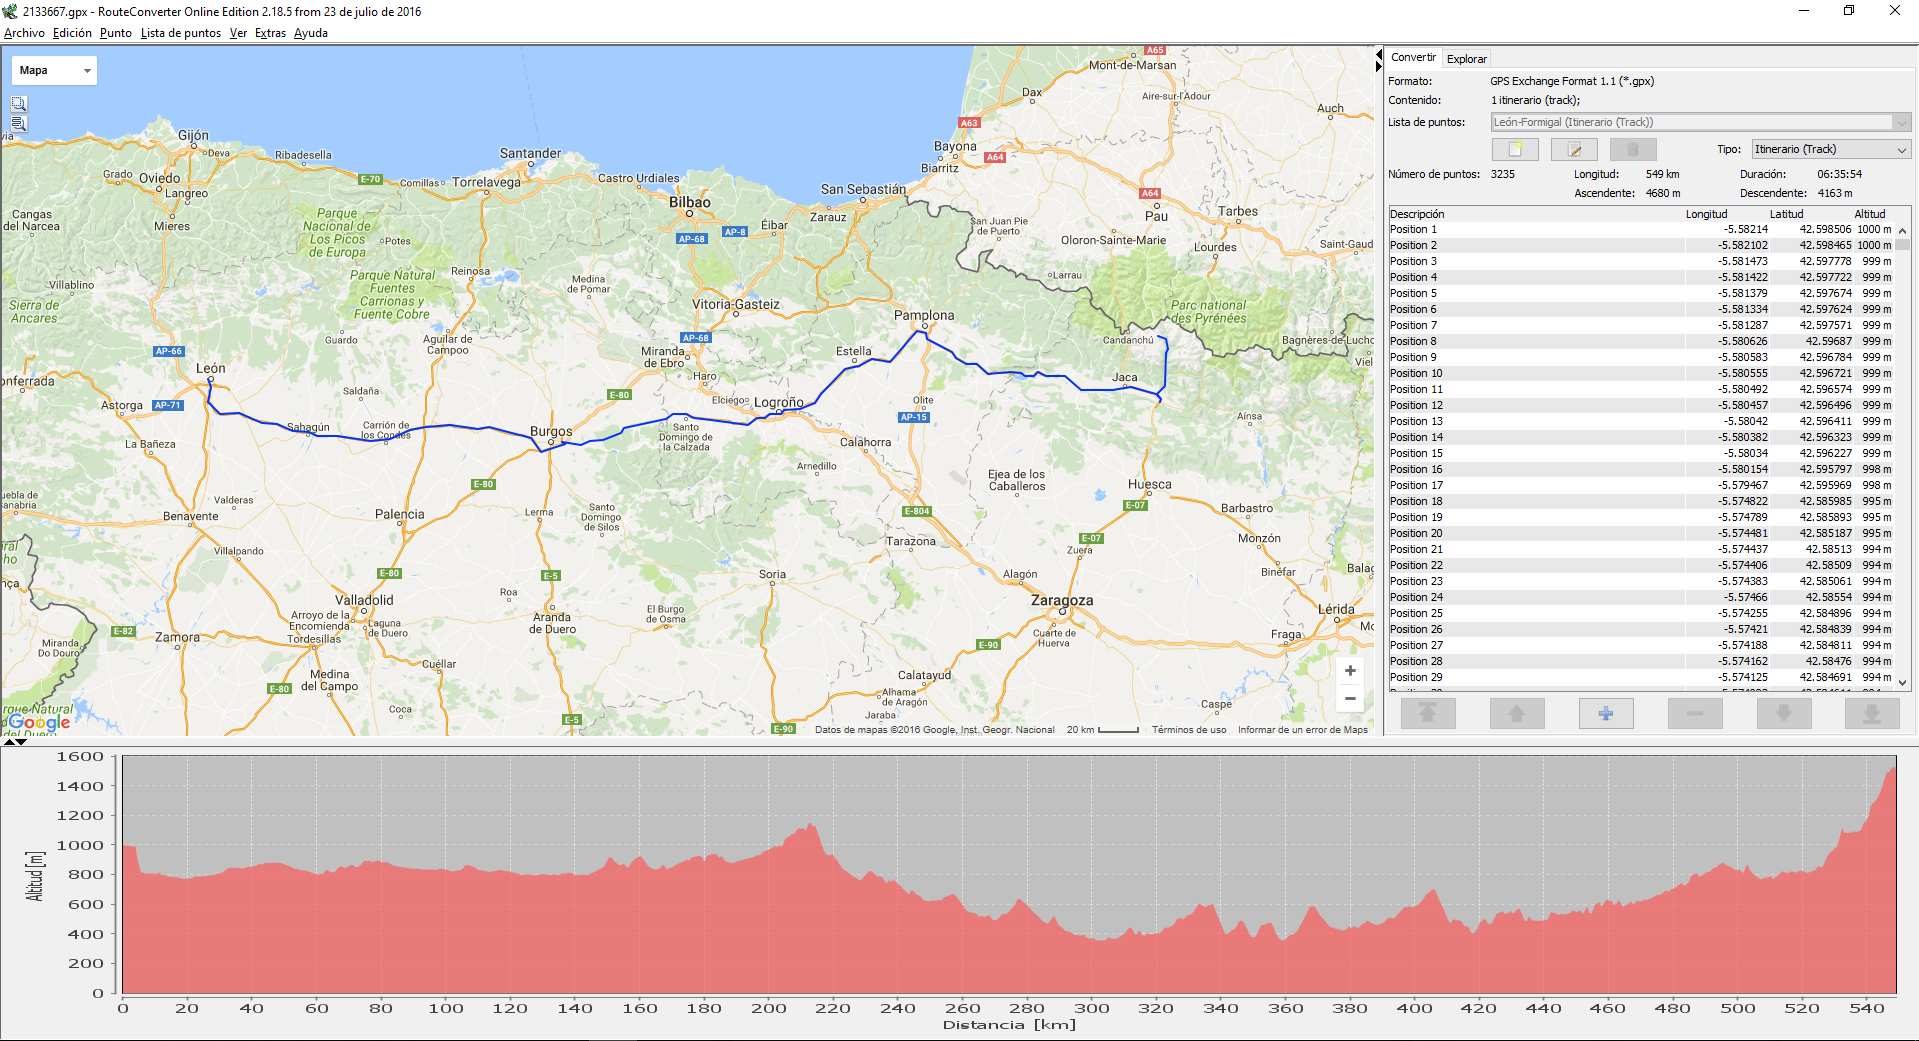
\includegraphics[width=0.8\textwidth]{../img/routeconverter/analisis_traza.png}
  \caption{Ruta desde León a Formigal}
  \label{rutaLeonFormigal}
\end{figure}

En la parte derecha de la ventana se pueden visualizar las rutas detectadas por el programa en el desplegable "Lista de puntos". En la parte inferior se listarán todos los puntos que conforman dicha lista como se ve en la Figura \ref{puntosGeograficos}.

\begin{figure}[h]
  \centering
    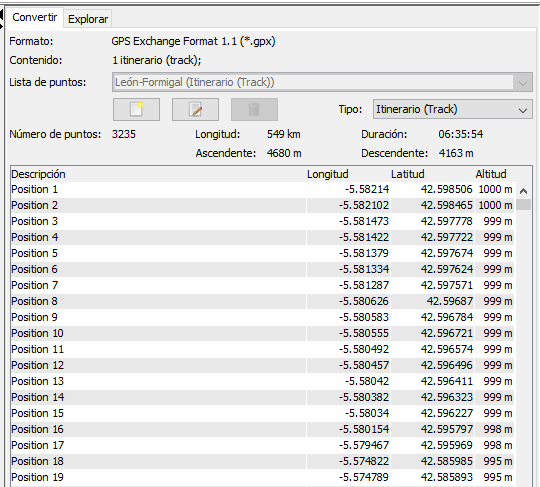
\includegraphics[width=0.6\textwidth]{../img/routeconverter/datos_traza.png}
  \caption{Ruta desde León a Formigal}
  \label{puntosGeograficos}
\end{figure}

Si la traza contiene elevaciones del terreno, se mostrará un perfil en la parte inferior.

